\documentclass{article}

\usepackage{fullpage,amsmath,amsthm,graphicx,enumitem}
\usepackage{hyperref}
\usepackage{amssymb}
\usepackage{wasysym}
\usepackage{color}
\usepackage[capitalize]{cleveref}

\newcommand{\todo}[1]{\textbf{\textcolor{red}{#1}}}

\theoremstyle{definition}
\newtheorem{task}{Task}
\crefname{task}{Task}{Tasks}

\newcommand{\option}{{\Large$\Square$ }}

\title{ASEN 3728 Aircraft Dynamics\\Programming Homework 1}

\date{Due date listed on Gradescope.}


\begin{filecontents}{bibliography.bib}
@inproceedings{weixuan_zhang_controllable_2016,
	title = {A controllable flying vehicle with a single moving part},
	url = {http://ieeexplore.ieee.org/document/7487499/},
	eventtitle = {2016 {IEEE} International Conference on Robotics and Automation ({ICRA})},
	pages = {3275--3281},
	booktitle = {2016 {IEEE} International Conference on Robotics and Automation ({ICRA})},
	author = {{Weixuan Zhang} and Mueller, Mark W. and D'Andrea, Raffaello},
    year = {2016},
}
\end{filecontents}

\begin{document}

\maketitle

In this assignment, you will write a Matlab program to simulate the dynamics of a monospinner vehicle\cite{weixuan_zhang_controllable_2016}. The monospinner is a flying machine with a single moving part. At one end, at a length $l$ from the center of mass along the $x$ axis, it has a propeller that produces an aerodynamic thrust, $f_P$, in the $-z$ direction and moment, $\tau_P$ about the $-z$ direction. The control input is the thrust $\textbf{u} = [f_P]$, and the moment is proportional to this thrust: $\tau_P = k_m f_P$. Numerical values for all of the constants are contained in the code templates. The rest of the electronics are placed carefully to produce dynamics that allow the vehicle to fly with a spinning motion that can be seen in the video here: \url{https://www.youtube.com/watch?v=P3fM6VwXXFM}.

\begin{figure}[h]
\centering
\begin{minipage}{0.9\textwidth}
\begin{minipage}{0.5\textwidth}
        \centering
        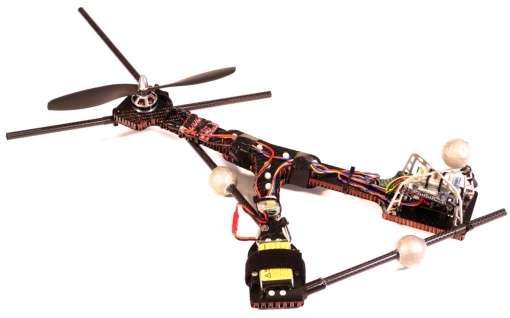
\includegraphics[width=\textwidth]{monospinner.pdf}
        \caption{The monospinner vehicle.}
\end{minipage}
\begin{minipage}{0.5\textwidth}
        \centering
        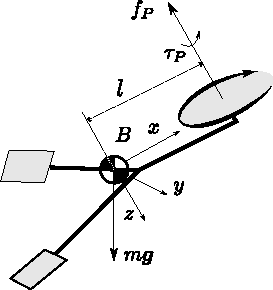
\includegraphics[width=0.6\textwidth]{monospinner-coordinates.pdf}
        \caption{Coordinates, forces, and moments.}
\end{minipage}
\end{minipage}
\end{figure}

All files are available by cloning the git repository at \url{https://github.com/zsunberg/Aircraft-Dynamics-Materials} and navigating to the \texttt{assignments/P1} directory. A zip file is also available at \url{https://github.com/zsunberg/Aircraft-Dynamics-Materials/raw/main/zips/assignments/P1.zip}. It is possible that there will be bugfixes to the assignment after it is released. These will be announced on Piazza.

\begin{task}
    Create the \texttt{rotation321} function that returns the rotation matrix $R^B_E$ given a vector of the Euler angles $\phi$, $\theta$, and $\psi$. You can test this function by running the command \texttt{run(testRotation321)} in Matlab. The file \texttt{TEMPLATE\_rotation321.m} contains a template for this function.
\end{task}

\begin{task}
    Create the Matlab function \texttt{attitudeInfluence321} that returns the attitude influence matrix, $T$, given a vector of the Euler angles $\phi$, $\theta$, and $\psi$. You can test this function by running the command \texttt{run(testAttitudeInfluence321)} in Matlab. The file \texttt{TEMPLATE\_attitudeInfluence321.m} contains a template for this function.
\end{task}

\begin{task}
    Create the Matlab function \texttt{monospinnerDynamics} that returns the state derivative $\dot{\textbf{x}}$ given the time $t$, state $\textbf{x}$, and control input $\textbf{u}$. You can test this function by running the command \texttt{run(testMonospinnerDynamics)} in Matlab. The file \texttt{TEMPLATE\_monospinnerDynamics.m} contains a template for this function. You do not need to include aerodynamic forces or moments other than those created by the idealized rotor model described above.
\end{task}

\begin{task}
    In Matlab, run the command \texttt{evaluate('your.gradescope.email@colorado.edu')} (replacing the email address with the one you use for Gradescope). This will run the tests on your code and produce a file called \texttt{submission.json} that certifies that your code passes the tests. You will upload \texttt{submission.json} to Gradescope to receive credit for this assignment.
\end{task}

\begin{task}\label{task:powered}
    Using \texttt{ode45}, simulate the monospinner dynamics for 5 seconds with a constant thrust of 2.3 N, $\textbf{u}=[2.3]$, starting from a zero initial condition. Plot the position, attitude, velocity, and angular rate of the monospinner over time by modifying and calling the function in the \texttt{TEMPLATE\_plotStateHistory.m} file. Which angular rate initially grows the fastest? Why?
\end{task}

\begin{task}\label{task:ballistic}
    Using \texttt{ode45}, simulate the monospinner dynamics for 5 seconds with no thrust, $\textbf{u}=[0]$ starting from the initial condition $\textbf{x}(0) = [0; 0; 0;\,  0; 0; 0;\, 1; 1; -20;\, 0; -5; 0]$. Plot the position, attitude, velocity, and angular rate of the monospinner over time by modifying and calling the function in the \texttt{TEMPLATE\_plotStateHistory.m} file. Since the only force acting on the monospinner is gravity, it should follow a ballistic trajectory meaning that the downward velocity should increase linearly with time. Why does the velocity term $w$ oscillate? Since there are no torques acting on the monospinner, the angular momentum should be constant. Why do the angular rate components $p$, $q$, and $r$ oscillate?
\end{task}

\begin{task}\label{task:aero}
    In the model you coded for this assignment, it would likely be impossible to stabilize the monospinner to steady state flight. What real-life forces and/or moments were not modeled that make it possible for the real monospinner to reach steady state flight? Why are they needed?
\end{task}

\subsection*{Deliverables}
In order to use the template files, rename them by removing \texttt{TEMPLATE\_}. To produce the report with plots and question answers, using the Matlab command \texttt{publish('report.m', 'pdf')} is highly recommended. Submit the following files to Gradescope:
\begin{itemize}[noitemsep]
    \item \texttt{submission.json} (make sure that the Gradescope autograder runs successfully when you submit!)
    \item \texttt{report.pdf} containing plots and answers to the questions (a couple sentences each) for \cref{task:powered,task:ballistic,task:aero}.
    \item \texttt{rotation321.m}
    \item \texttt{attitudeInfluence321.m}
    \item \texttt{monospinnerDynamics.m}
    \item \texttt{plotStateHistory.m}
\end{itemize}

\bibliographystyle{IEEEtran}
\bibliography{bibliography}

\end{document}
